\section{Introduction to thermal imaging}

Thermal imaging is a technique that utilizes infrared radiation emitted from nearly any objects. 
The existence of infrared radiation was first discovered in 1800 by Sir Frederick William Herschel. 
His experiments lead to the knowledge that there is a light spectrum beyond the visual spectrum humans are able to perceive. Any object above absolute zero emits energy-electromagnetic radiation depending on its temperature.\cite{ignacio2017,optris2009}

Infrared radiation is also known as thermal radiation because of the relationship between temperature and infrared radiation. Temperature of the human body permits radiation in the infrared spectrum, but objects of much higher temperature are capable of emitting radiation in the visible and UV spectrum. This has to do with the difference between object and environmental temperature. If the temperature of these are relatively close to each other, the radiation emitted will be within infrared wavelengths. Infrared radiation has a wavelength from 769 nm to 1 mm. Objects emit more radiation in some regions compared to others. Because of this the infrared spectrum is classified in the three regions, near (769 nm - 2.5 $\mu$m), middle (2.5 $\mu$m - 50 $\mu$m) and far infrared (50 $\mu$m - 1 mm). The human body emits most radiation in the far infrared spectrum. Near and middle cameras are mainly used to measure gases.\cite{ignacio2017}

Thermal imaging is commonly used to calculate surface temperatures. Two important concepts, heat and temperature emerge in the understanding of this. Temperature is a measure for the internal energy within an object and can be defined as the average kinetic energy of the object.
Heat is the energy that passes from a warm object to a colder object. Warm objects will decrease in internal energy and cold objects will increase due to the temperature difference and therefore the heat transfer. In the human body, a constant temperature is kept, homeostasis and therefore the temperature will not decrease even though a heat transfer to the surrounding environment occurs. The environmental temperature do have an impact on how large the heat transfer gradient is. If a body is in a cold environment, the emitted heat will be greater than the absorbed. In the same way, if the environment is much warmer than 37$^{\circ}$C, a greater absorption than emission will occur and the body will increase in temperature.\cite{ignacio2017} 

\section{Measuring thermal energy}

The theory of the black body is important to understand the absorption and emission of radiation relative to temperature. Because the theory of the black body is used to describe the laws of infrared radiation and its relationship to temperature. The black body is an ideal perfect emitter of infrared radiation because it absorbs all electromagnetic radiation permitted to it. The black body emits the same amount of radiation as it absorbs, the absorption and emission are both equal to one. 
Spectral emissive power, also denoted $E_\lambda$ is the energy emitted by a surface in relation to time and range of wavelength. Figure \ref{fig:Spectral} shows a graphical illustration of spectral emissive power of the black body for specific wavelengths when the temperature changes. \cite{ignacio2017} 

\begin{figure}[H]
	\centering	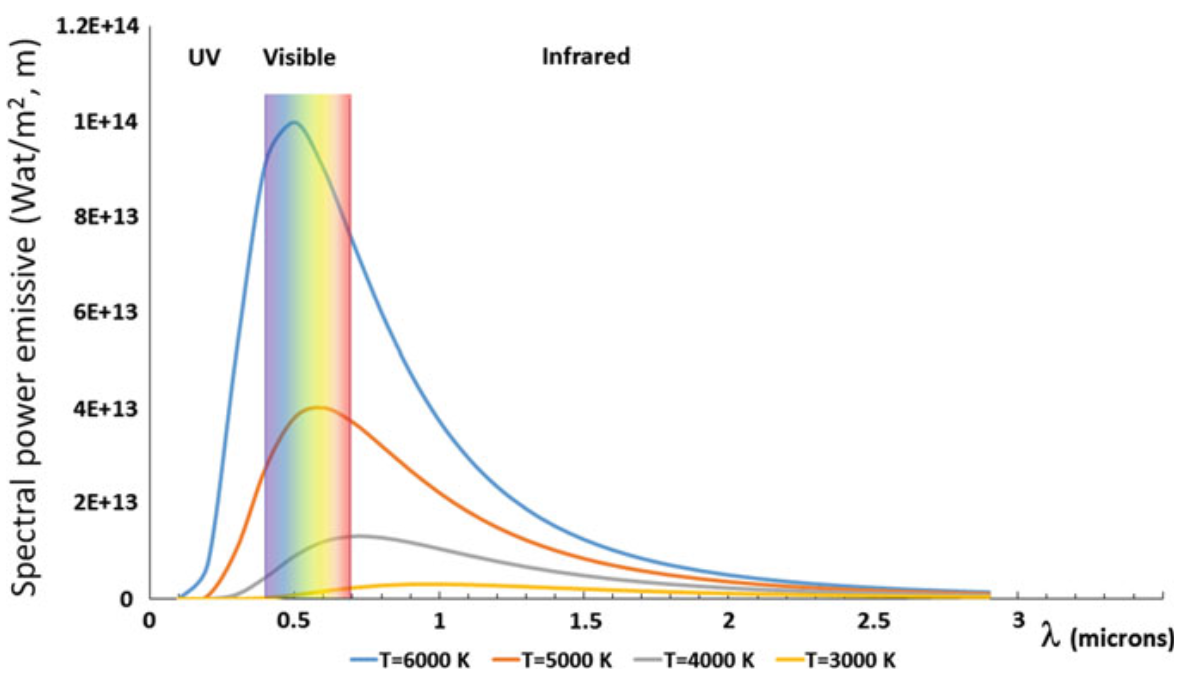
\includegraphics[width=0.7\textwidth]{figures/Spectral_power_emissive}
	\caption{Spectral power emissive as a function of wavelength for different temperatures.\cite{ignacio2017}}
	\label{fig:Spectral}
\end{figure} \vspace{-.3cm}

The knowledge of this principle helps in the understanding of how infrared radiation behaves, and how temperature affects the wavelength of the signal. 
The radiation from the human body which has a temperature at 37$^{\circ}$C emits the maximum energy of $9.3 \mu$m.\cite{ignacio2017}

Physical laws including Wien's displacement law and Stefan-Boltzmann's law are important for explaining how the infrared radiation behaves at different temperatures. \cite{ignacio2017} 

Wien's displacement law explains that the wavelength of the peak of the black body radiation curve decreases as the body temperature increases. This law can be used to describe different wavelengths according to the temperature of the black body which emits the radiation. Wien's law has the following equation:\cite{ignacio2017} 

\begin{flalign}
	\lambda_{max} = \frac{a}{T}
	\label{eq:wien}
\end{flalign}

$a$ has a value of $2.897*10^{-3} m K$ and denotes the Wien's displacement constant. $T$ denotes the absolute temperature in kelvin. $\lambda_{max}$ denotes the wavelength of emission peak with unit in meters.\cite{ignacio2017} 

Stefan-Boltzmann's law explains that small changes in temperature will lead to big changes in emissive power. This is seen in Stefan-Boltzmann's equation because it states that the total emissive power is proportional to the fourth power of the absolute  temperature. \cite{ignacio2017}

\begin{flalign}
	E = {\varepsilon}*{\sigma}*{T^4}
	\label{eq:stefan}
\end{flalign}

In Stefan-Boltzmann's equation $E$ denotes the total emissive power with unit $W/m^{2}$. $\sigma$ denotes the Stefan-Boltzmann's constant, and has a value of $5.67*10^{-8} W/m^{-2} K^{-4}$. $T$ is the temperature in kelvin. $\varepsilon$ denotes the emissivity and is normally not a part of the Stefan-Boltzmann's law, but part of the modified Stefan-Boltzmann's equation, because it is used for calculation of temperature in most thermal cameras.\cite{ignacio2017}

Emissivity is different for all materials. Skin has an emissivity between 0.95 and 0.99, why these values typically are used when assessing the temperature of the skin of the human body with thermal imaging.
This law is important when considering thermal imaging because the sensitivity when calculating the temperature from the emissive power is considerable.\cite{ignacio2017}


\subsection{Thermal cameras} \label{sec:cam}

Thermal cameras contain a lens to focus the electromagnetic radiation emitted by an object onto a detector element. A focal plan array (FPA) contains between $384\times 288$ and $1024\times 768$ microbolometers and is often used as detector element in uncooled thermal cameras.\cite{olbrycht2015,optris2009} 
The thermal radiation focused by the lens warms up the microbolometers in the FPA. This warming is proportional to the detected radiation. Since microbolometers contain temperature-dependent electric resistance, the voltage of the electrical outcome signal is depending on the detected radiation.
The infrared radiation is detected as an analogue signal by the FPA. An AD-converter prepares the signal for the processor module in the thermal camera. The signal is modified into pixels, what gives a digital image as an output, which contains the temperature informations of the observed object. A schematic representation of this is illustrated on figure \ref{fig:em_spectrum}. \cite{optris2009,ignacio2017}

\begin{figure}[H]                                         
	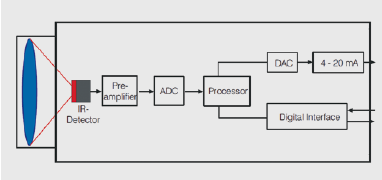
\includegraphics[width=.55\textwidth]{figures/IR_cam}  
	\caption{Simplified buildup a standard thermal detector.\cite{optris2009}}
	\label{fig:em_spectrum}  
\end{figure} 









%\section{Physical principals}
%
%Any object above absolute zero emits energy-electromagnetic radiation depending on its temperature. Absolute zero is $0K$ or $ -273.16^{\circ}$C. To put that into perspective the human body has a temperature around 37$^{\circ}$C.\cite{ignacio2017,optris2009}
%
%Electromagnetic radiation is a propagation of energy trough a medium without the transportation of mass. An electromagnetic wave is made of the relationship between frequency $f$, wavelength $\lambda$ and the speed of light $c$. This is stated in the equation of wave motion.\cite{ignacio2017}  
%\begin{flalign}
%	\lambda = \frac{c}{f}
%	\label{eq:wave}
%\end{flalign}
%Depending on the frequency and wavelength certain characteristics arise from what is called the electromagnetic spectrum. The electromagnetic spectrum is the electromagnetic energy that is emitted. This extends from radiation of low energy such as radio waves and infrared, to waves of higher energy in form of eg. X-rays. A graphical representation of the electromagnetic spectrum can be seen on \cref{fig:em_spectrum}.\cite{ignacio2017}        
%
%\begin{figure}[H]                                         
%	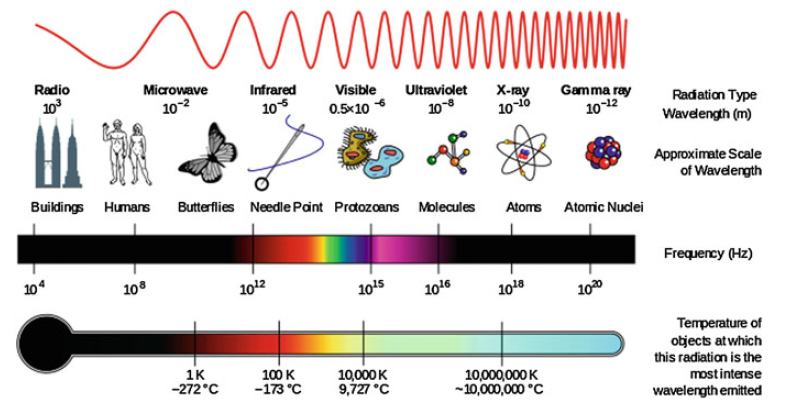
\includegraphics[width=.66\textwidth]{figures/em_spectrum}  
%	\caption{The electromagnetic spectrum with wavelength, emitters, frequency and temperature.\cite{ignacio2017}}
%	\label{fig:em_spectrum}  
%\end{figure}   
%
%Infrared radiation is also known as thermal radiation because of the relationship between temperature and infrared radiation. Temperature of the human body permits radiation in the infrared spectrum, but objects of much higher temperature are capable of emitting radiation in the visible and UV spectrum. This has to do with the difference between object and environmental temperature. If the temperature of these are relatively close to each other, the radiation emitted will be within infrared wavelengths. Infrared radiation has a wavelength from 769 nm to 1 mm. Objects emit more radiation in some region regions compared to others. Because of this is the infrared spectrum classified in the three regions, near, middle and far infrared. Near is between 769 nm and 2.5 $\mu$m, middle 2.5 $\mu$m to 50 $\mu$m and far 50 $\mu$m to 1 mm. The human body emits most radiation in the far infrared part, and most thermal cameras are build with this in mind. Near and middle cameras are used to measure gases.\cite{ignacio2017} 
%
%
%
%
%%A bit more needs to be written here i think..
%%
%%
%%Extra notes that i'we just copied that we can use later 
%%
%%The advantages of non-contact temperature measurement
%%are obvious – it supports:
%%
%%• Temperature measurements of moving or overheated
%%objects and of objects in hazardous surroundings
%%
%%• Very fast response and exposure times
%%
%%• Non-interactive measurement, no influence on
%%the measuring object
%%
%%• Non-destructive measurement
%%
%%• Measurement point durability, no mechanical wear




